
\documentclass[border=10pt]{standalone}
\usepackage{tikz}
\usepackage{pgfplots}
\pgfplotsset{compat=1.18}
\begin{document}
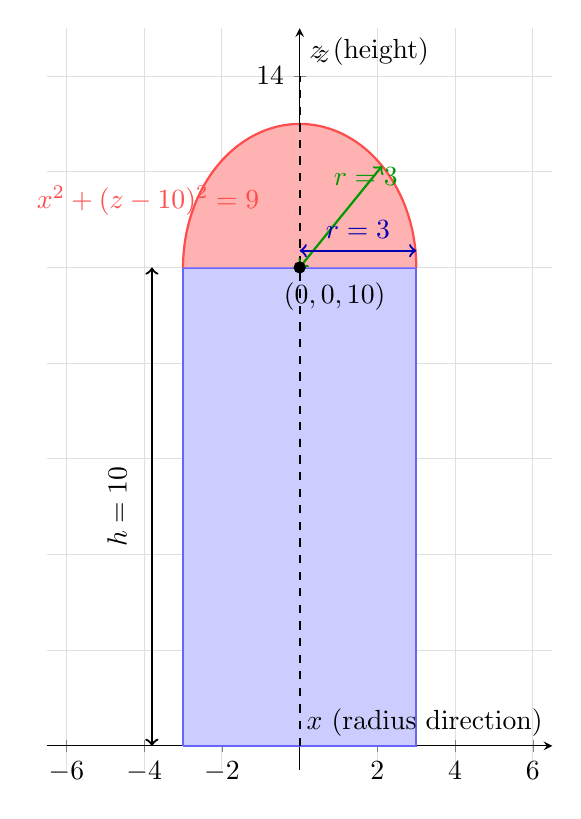
\begin{tikzpicture}
\begin{axis}[
    width=8cm, height=11cm,
    xlabel=$x$ (radius direction), ylabel=$z$ (height),
    xmin=-6.5, xmax=6.5, ymin=-0.5, ymax=15,
    axis lines=middle,
    ytick={0,2,4,6,8,10,12,14},
    xtick={-6,-4,-2,0,2,4,6},
    grid=both, grid style={gray!25},
    clip=false,
]
% ---- Cylinder cross-section: rectangle ----
\addplot[fill=blue!20, draw=blue!60, thick] coordinates {(-3,0) (3,0) (3,10) (-3,10) (-3,0)};
% ---- Hemisphere cross-section: semicircle ----
\addplot[fill=red!30, draw=red!70, thick, domain=0:180, samples=100]
    ({3*cos(x)}, {10 + 3*sin(x)});
% ---- z axis dashed ----
\addplot[dashed, black, thick, domain=0:14] ({0}, {x});
% ---- radius on dome ----
\addplot[green!60!black, thick, <->, domain=0:1] ({3*x*cos(45)}, {10 + 3*x*sin(45)});
\node[green!60!black] at (axis cs:1.7,11.9) {$r=3$};
% ---- radius at cylinder top ----
\addplot[blue!70!black, thick, <->] coordinates {(0,10.35) (3,10.35)};
\node[blue!70!black] at (axis cs:1.5,10.8) {$r=3$};
% ---- height h=10 ----
\addplot[black, thick, <->] coordinates {(-3.8,0) (-3.8,10)};
\node[black, rotate=90] at (axis cs:-4.7,5) {$h=10$};
% ---- labels ----
\node at (axis cs:-3.9,11.4) {\color{red!70}$x^2+(z-10)^2=9$};
\node at (axis cs:0.9,9.4) {$(0,0,10)$};
\addplot[only marks, mark=*, black] coordinates {(0,10)};
\node at (axis cs:0.6,14.4) {$z$};
\end{axis}
\end{tikzpicture}
\end{document}
